\documentclass{article}

\usepackage{geometry}
\usepackage[T1]{fontenc}
\usepackage[utf8]{inputenc}
\usepackage{amssymb}
\usepackage{amsmath}
\usepackage{german}

\usepackage{tikz}

\usepackage{listings}
\usepackage{color}

\begin{document}
	
	\section{Rechenoperationen}
	\begin{enumerate}
		\item Baum besteht aus Knoten (Kreise) und Kanten (Pfeile)
		\item Kanten verbinden Knoten mit ihren Kind-Knoten
		\item jeder Knoten (außer der Wurzel) hat \underline{genau ein} Elternteil
		\item Knoten ohne Kinder heißen "'Blätter"' (leaf-nodes)
		\item Teilbaum
		\begin{enumerate}
			\item wähle beliebigen Knoten
			\item entferne temporär dessen Eltern-Kante
			\begin{enumerate}
				\item der Knoten wird temorär zu einer Wurzel
				\item dieser Knoten mit allen seinen Nachkommen bildet wieder seinen Baum - "' Teilbaum des Originalbaums"'
			\end{enumerate}
			\item Tiefe: Abstand des Knotens zur Wurzel
			\item 
		\end{enumerate}
	\end{enumerate}
	
	Infix-Notation: \\
	 $1+2+3*4/(1+5)-2$ \\ \\
	 Präfix-Notation: \\
	 $sub(add(add(1,2), div(mul(3,4), add(1,5))),2)$ \\ \\
	 
	 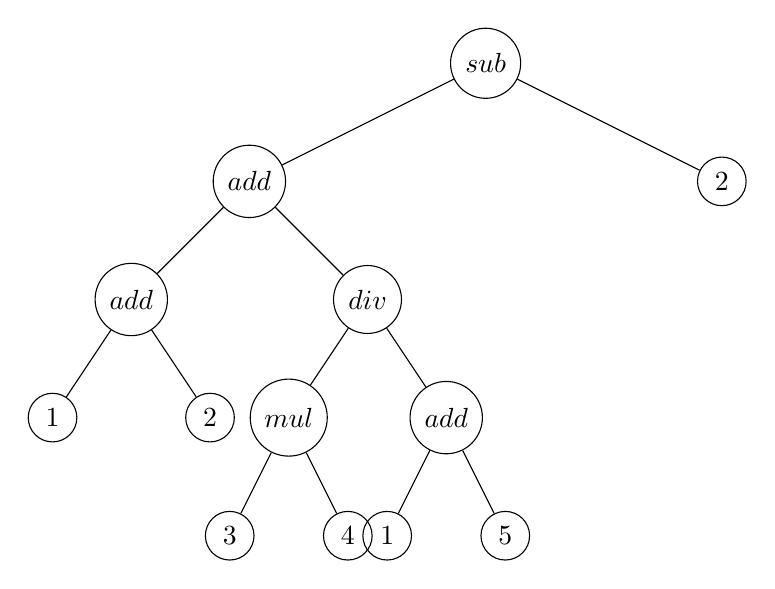
\begin{tikzpicture}[level/.style={sibling distance=60mm/#1}]
	 	
	 	\node [circle, draw] (z)  {$sub$}
	 	child {node [circle, draw] {$add$}
	 		child {node [circle, draw] {$add$}
	 			child{node [circle, draw] {$1$}}
	 			child{node [circle, draw] {$2$}}
	 		}
	 		child {node [circle, draw] {$div$}
	 			child{node [circle, draw] {$mul$}
	 				child {node [circle, draw] {$3$}}
	 				child {node [circle, draw] {$4$}}
	 			}
	 			child{node [circle, draw] {$add$}
	 				child {node [circle, draw] {$1$}}
	 				child {node [circle, draw] {$5$}}
	 			}
	 		}}
	 		child {node [circle, draw] {$2$}
	 		};
	 	\end{tikzpicture}
	 		
	\paragraph{Präfix Notation aus dem Baum rekonstruieren}
	 		
	 \begin{enumerate}
	 	\item Wenn die Wurzel ein Blatt ist, dann "'Drucke die Zahl"'
	 	\item sonst (Operator):
	 	\begin{enumerate}
	 		\item Drucke Funktionsnamen
	 		\item Drucke "'("'
	 		\item wiederhole ab $1)$ für das linke Kind
	 		\item Drucke "',"'
	 		\item wiederhole den Algorithmus ab $1)$ für das rechte Kind
	 		\item Drucke "')"'
	 	\end{enumerate}
	 \end{enumerate}
	
		Beachte Reihenfolge: Wurzel - Links - Rechts (Pre-Order Traversal)
		Ergebnis: \\
		$sub(add(add(1,2), div(mul(3,4), add(1,5))),2)$
		
		\paragraph{Definition: Rekursion}
		Rekursion meint Algorithmus für Teilproblem von vorn
		
		\paragraph{Infix Notation}
		
		\begin{enumerate}
			\item wie bei Präfix
			\item sonst
			\begin{enumerate}
				\item entfällt
				\item wie bei Präfix
				\item wie bei Präfix
				\item Drucke Operatorsymbol
				\item wie bei Präfix 
				\item wie bei Präfix
				\item wie bei Präfix
			\end{enumerate}
		\end{enumerate}
		Beachte Reihenfolge: Links - Wurzel - Rechts (In-Order Traversal) \newline
		
		Ergebnis: \\
		$(((1 + 2) + ((3 * 4)/(1 + 5))) + 2)$
		
		\paragraph{Berechne den Wert mit Substitutionsmethode}
		\begin{enumerate}
			\item Wenn Wurzel ein Blatt hat, gib die Zahl zurück
			\item sonst
			\begin{enumerate}
				\item entfällt
				\item entfällt
				\item wiederhole ab $1)$ für linken Teilbaum und speichere Ergebnis als "'left-result"'
				\item entfällt
				\item wiederhole ab $1)$ für rechten Teilbaum, speichere Ergebnis als "'right-result"'
				\item berechne $fkt_name(left-result, right-result)$ und gib Ergebnis zurück
			\end{enumerate}
		\end{enumerate}
		Beachte Reihenfolge: Links - Rechts - Wurzel (Post-Order Traversal)
		
		\begin{align*}
		&  	sub(add(add(1,2), div(mul(3,4), add(1,5))),2) \\
		= & \, sub(add(add(1,2), div(12, 6)),2) \\
		= & \, sub(add(3,2)2) \\
		= & \, sub(5,2) \\
		= & \, 3
		\end{align*}
		
		\section{Maschinensprache}
		\begin{itemize}
			\item optimiert für die Hardware (viele verschiedene)
			\item Gegensatz: höhere Programmiersprache ($C++$) ist optimiert für Programmierer
			\item Compiler oder Interpreter übersetzen Hoch- in Maschinensprache 
		\end{itemize}
		
		\paragraph{Vorgang des Übersetzens}
		\begin{enumerate}
			\item Eingaben (und Zwischenergebnisse) werden in Speicherzellen abgelegt $ \Rightarrow$ jeder Knoten im Baum bekommt eine Speicherzelle (Maschinensprache: durchnumeriert ; Hochsprache: sprechende Namen)
			\item Speicherzellen für die Eingaben $\underline{initialisieren}$ ; Notation: SpZ $\leftarrow$ Wert
			\item Rechenoperationen in der Reihenfolge des Substitutionsmodells ausführen und in der jeweiligen Speicherzelle speichern ; Notation: SpZ\_Ergebnis $\leftarrow$ fkt\_name SpZ\_Arg1 SpZ\_Arg2
			\item alles in Zahlencode umwandeln
			\begin{itemize}
				\item Funktionsname $\Rightarrow$ Opcodes
				\item Speicherzellen: nur die Nummer
				\item Werte sind schon Zahlen
				\item Notation: Opcode \quad Ziel SpZ \quad SpZ\_Arg1 \quad SpZ\_Arg2 oder Opcode \quad Ziel SpZ \quad Initialwert
			\end{itemize}
		\end{enumerate}
	
	\section{funktionale Programmierung}
	(alles durch Funktionsaufrufe ausführen)
	
	\begin{enumerate}
		\item bei Maschinensprache wurden Zwischenergebnisse in Speicherzellen abgelegt
		\item das ist auch in der funktionalen Programm. eine gute Idee
		\begin{enumerate}
			\item Speicherzellen werden durch Namen (vom Programmierer vergeben) unterschieden
			\item Beispiel: Lösen einer quadratischen Gleichung: $ax^2+bx+c =0$, finde $x_{1/2}$
					$\Rightarrow x^2-px+q =0 \quad mit \quad p = -\frac{b}{2a}, q = \frac{c}{a}$
					$\Rightarrow x_1 = -\frac{b}{2a} + \sqrt{(-\frac{b}{2a}^2 - \frac{c}{a})} \\ \Leftarrow allgemein: x_{1/2} = p \pm \sqrt{p^2-q}$
			\item Präfix: \\ $x_1 \leftarrow add(div(div(b,a),-2), sqrt(sub(mul(div(div(b,a),-2), div(div(b,a), -2)), div(c,a))))$ \\
					mit Zwischenergebnissen und Infix-Notation: $p \leftarrow b/c/-2 \quad $oder$ \quad p \leftarrow -0,5*b/a \quad q \leftarrow c/a$ \\ $discriminant \leftarrow sqrt(p*P-q)$ \\
					$x_{1/2} \leftarrow p \pm discriminant$
		\end{enumerate}
		\item zwei Vorteile:
		\begin{enumerate}
			\item lesbar
			\item redundante Berechnung verschieden \\ Beachte: In der funktionalen Programmierung können die Speicherzellen nach der Initialisierung \underline{nicht} mehr verändert werden
			\item Speicherzellen mit Namen sind nützlich, um Argumente an Funktionen zu übergeben $\Rightarrow$ Definition eigener Funktionen \\
			Bsp: 
			\framebox{function sq(x) \\
												\{
												return x*x
												\} }
		\end{enumerate}
	\end{enumerate}
	
	\section{funktionale Programmierung in C++}
	
	\begin{enumerate}
		\item in C++ hat jede Speicherzelle einen \underline{Typ} (legt Größe und Bedeutung der Speicherzelle fest) \\
		wichtigste Typen: \grqq int\grqq  für ganze Zahlen, \grqq double\grqq  für reelle Zahlen, \grqq std::string\grqq  für Text \\ zugehörige Literale (Konstanten): 12, -3 (int) \quad -1.02 , 1.2e-4 (double) \quad \grqq text text \grqq (string)
		\item Die Initialisierung wird geschrieben als
		\begin{lstlisting}[tabsize =2]
			type_name spz_name = initialwert
		\end{lstlisting}
		Bsp:
		\begin{lstlisting}[tabsize = 2]
			double a = 10
			std::cout << "x_1" << x_1 << "\n" ;
		\end{lstlisting} 
		\item eigene Funktion in $C++$: 

			\begin{lstlisting}[tabsize = 2]
			type_ergebnis funktionsname (typ_arg1 name_arg1, typ_arg2 name_arg2)
			{
				<code>
				return ergebnis;
			}
			\end{lstlisting}
			
		\item zwei Funktionen mit gleichem Namen, aber unterschiedlichen Typen dürfen in C++ gleichzeitig definiert sein (\grqq overloading\grqq) \\ $\Rightarrow$ C++ wählt \underline{automatisch} die richtige Variante anhand des Argumenttypes (\grqq overload resolution\grqq)
		
		\item jedes $C++$ -Programm muss \underline{genau eine} Funktion names \grqq main\grqq haben: Dort beginnt die Programm-Ausführung \\
		Bsp: \\
		\fbox{\centering int main() \{ <code> \quad return 0 (erfolgreich abgearbeitet)\}}
		
		\item Regel von $C++$ für erlaubte Namen (Speicherzelle \& Funktion):
		\begin{enumerate}
			\item erste Zeichen: Klein- oder Großbuchstaben des englischen Alphabets oder \_
			\item optional: weitere Zeichen: wie erstes Zeichen oder Ziffern 0 \dots 9
		\end{enumerate}
		
		\item vordefinierte Funktionen in $C++$
		\begin{enumerate}
			\item eingebaute Funktionen (immer vorhanden) z.B. Infix Operatoren
			\item Funktionen der Standardbibliothek (Programmierer muss sie explizit auffordern)
			\begin{enumerate}
				\item z.B. algebraische Funtionen beginnend mit std::\dots
				\item sind in Module geordnet, z.B. cmath $\widehat{=}$ \, algebraische Funktionen, iostream $\widehat{=}$ \, Ausgabe, z.B. std::cout
				\item Um ein Modul zu benutzen, muss man zuerst (am Anfang des Programms) sein Inhaltsverzeichnis importieren \\
				\frame{\centering \#include <module\_name>} sprich \grqq Header inkludieren\grqq \\
				 \\
			\end{enumerate}
		\end{enumerate}
	\end{enumerate}
	
	\begin{lstlisting}
	# include <iostream> 
	# include <string> 
	
	int main() {
	
	std::cout <<  "Hello" << "\n";
	std::string >> ausgabe = "mein erstes Programm"
	std::cout << ausgabe;
	
	return 0
	}
	\end{lstlisting}
	
	\paragraph{Overloading der arithmetischen Operationen}
	
	\begin{lstlisting}
		int a = 3;
		int b = 4;
		int c = a * b;
		double x = 3.0;
		double y = 4.0;
		double z = x * y;
	\end{lstlisting}
	$3.0 * 4 \quad \Rightarrow \quad$ automatische Umwandlung in höheren Typ, hier: \grqq double\grqq $\Rightarrow$ wird als $3.0 * 4.0$ ausgeführt \\
	
	Konsequenzen:
	\begin{enumerate}
		\item Division unterscheidet sich nach dem Datentypen: $(-12)/5 \Rightarrow -2 \neq -2.4 \Leftarrow (-12.0/5.0)$
		\item negative Ereignisse werden aufgerund, positive abgerundet
		\item Gegensatz (z.B. zu Python): floor division $\widehat{=}$ wird immer abgerundet
	\end{enumerate}
	
	
	
\end{document}